%
\begin{isabellebody}%
\setisabellecontext{Lens{\isacharunderscore}Laws}%
%
\isamarkupsection{Core Lens Laws%
}
\isamarkuptrue%
%
\isadelimtheory
%
\endisadelimtheory
%
\isatagtheory
\isacommand{theory}\isamarkupfalse%
\ Lens{\isacharunderscore}Laws\isanewline
\isakeyword{imports}\ \isanewline
\ \ Two\ Interp\isanewline
\isakeyword{begin}%
\endisatagtheory
{\isafoldtheory}%
%
\isadelimtheory
%
\endisadelimtheory
%
\isamarkupsubsection{Lens signature%
}
\isamarkuptrue%
\isacommand{record}\isamarkupfalse%
\ {\isacharparenleft}{\isacharprime}a{\isacharcomma}\ {\isacharprime}b{\isacharparenright}\ lens\ {\isacharequal}\isanewline
\ \ lens{\isacharunderscore}get\ {\isacharcolon}{\isacharcolon}\ {\isachardoublequoteopen}{\isacharprime}b\ {\isasymRightarrow}\ {\isacharprime}a{\isachardoublequoteclose}\ {\isacharparenleft}{\isachardoublequoteopen}get{\isasymindex}{\isachardoublequoteclose}{\isacharparenright}\isanewline
\ \ lens{\isacharunderscore}put\ {\isacharcolon}{\isacharcolon}\ {\isachardoublequoteopen}{\isacharprime}b\ {\isasymRightarrow}\ {\isacharprime}a\ {\isasymRightarrow}\ {\isacharprime}b{\isachardoublequoteclose}\ {\isacharparenleft}{\isachardoublequoteopen}put{\isasymindex}{\isachardoublequoteclose}{\isacharparenright}\isanewline
\isanewline
\isacommand{type{\isacharunderscore}notation}\isamarkupfalse%
\isanewline
\ \ lens\ {\isacharparenleft}\isakeyword{infixr}\ {\isachardoublequoteopen}{\isasymLongrightarrow}{\isachardoublequoteclose}\ {\isadigit{0}}{\isacharparenright}%
\begin{isamarkuptext}%
\begin{figure}
  \begin{center}
    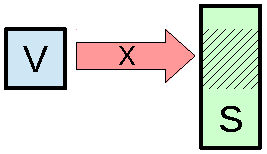
\includegraphics[width=3.5cm]{figures/Lens}
  \end{center}
  \vspace{-5ex}
  \caption{Visualisation of a simple lens}
  \label{fig:Lens}
  \end{figure}

  A lens $X : \view \lto \src$, for source type $\src$ and view type $\view$, identifies 
  $\view$ with a subregion of $\src$~\cite{Foster07,Foster09}, as illustrated in Figure~\ref{fig:Lens}. The arrow denotes 
  $X$ and the hatched area denotes the subregion $\view$ it characterises. Transformations on 
  $\view$ can be performed without affecting the parts of $\src$ outside the hatched area. The lens 
  signature consists of a pair of functions $\lget_X : \src \Rightarrow \view$ that extracts a view 
  from a source, and $\lput_X : \src \Rightarrow \view \Rightarrow \src$ that updates a view within 
  a given source.%
\end{isamarkuptext}\isamarkuptrue%
\isacommand{named{\isacharunderscore}theorems}\isamarkupfalse%
\ lens{\isacharunderscore}defs\isanewline
\isanewline
\isacommand{definition}\isamarkupfalse%
\ lens{\isacharunderscore}create\ {\isacharcolon}{\isacharcolon}\ {\isachardoublequoteopen}{\isacharparenleft}{\isacharprime}a\ {\isasymLongrightarrow}\ {\isacharprime}b{\isacharparenright}\ {\isasymRightarrow}\ {\isacharprime}a\ {\isasymRightarrow}\ {\isacharprime}b{\isachardoublequoteclose}\ {\isacharparenleft}{\isachardoublequoteopen}create{\isasymindex}{\isachardoublequoteclose}{\isacharparenright}\ \isakeyword{where}\isanewline
{\isacharbrackleft}lens{\isacharunderscore}defs{\isacharbrackright}{\isacharcolon}\ {\isachardoublequoteopen}create\isactrlbsub X\isactrlesub \ v\ {\isacharequal}\ put\isactrlbsub X\isactrlesub \ undefined\ v{\isachardoublequoteclose}%
\begin{isamarkuptext}%
Function $\lcreate_X~v$ creates an instance of the source type of $X$ by injecting $v$
  as the view, and leaving the remaining context arbitrary.%
\end{isamarkuptext}\isamarkuptrue%
%
\isamarkupsubsection{Weak lenses%
}
\isamarkuptrue%
%
\begin{isamarkuptext}%
Weak lenses are the least constrained class of lenses in our algebraic hierarchy. They
  simply require that the PutGet law~\cite{Foster09,Fischer2015} is satisfied, meaning that 
  $\lget$ is the inverse of $\lput$.%
\end{isamarkuptext}\isamarkuptrue%
\isacommand{locale}\isamarkupfalse%
\ weak{\isacharunderscore}lens\ {\isacharequal}\isanewline
\ \ \isakeyword{fixes}\ x\ {\isacharcolon}{\isacharcolon}\ {\isachardoublequoteopen}{\isacharprime}a\ {\isasymLongrightarrow}\ {\isacharprime}b{\isachardoublequoteclose}\ {\isacharparenleft}\isakeyword{structure}{\isacharparenright}\isanewline
\ \ \isakeyword{assumes}\ put{\isacharunderscore}get{\isacharcolon}\ {\isachardoublequoteopen}get\ {\isacharparenleft}put\ {\isasymsigma}\ v{\isacharparenright}\ {\isacharequal}\ v{\isachardoublequoteclose}\isanewline
\isakeyword{begin}\isanewline
\isanewline
\ \ \isacommand{lemma}\isamarkupfalse%
\ create{\isacharunderscore}get{\isacharcolon}\ {\isachardoublequoteopen}get\ {\isacharparenleft}create\ v{\isacharparenright}\ {\isacharequal}\ v{\isachardoublequoteclose}\isanewline
%
\isadelimproof
\ \ \ \ %
\endisadelimproof
%
\isatagproof
\isacommand{by}\isamarkupfalse%
\ {\isacharparenleft}simp\ add{\isacharcolon}\ lens{\isacharunderscore}create{\isacharunderscore}def\ put{\isacharunderscore}get{\isacharparenright}%
\endisatagproof
{\isafoldproof}%
%
\isadelimproof
\isanewline
%
\endisadelimproof
\isanewline
\ \ \isacommand{lemma}\isamarkupfalse%
\ create{\isacharunderscore}inj{\isacharcolon}\ {\isachardoublequoteopen}inj\ create{\isachardoublequoteclose}\isanewline
%
\isadelimproof
\ \ \ \ %
\endisadelimproof
%
\isatagproof
\isacommand{by}\isamarkupfalse%
\ {\isacharparenleft}metis\ create{\isacharunderscore}get\ injI{\isacharparenright}%
\endisatagproof
{\isafoldproof}%
%
\isadelimproof
\isanewline
%
\endisadelimproof
\isanewline
\ \ \isacommand{definition}\isamarkupfalse%
\ update\ {\isacharcolon}{\isacharcolon}\ {\isachardoublequoteopen}{\isacharparenleft}{\isacharprime}a\ {\isasymRightarrow}\ {\isacharprime}a{\isacharparenright}\ {\isasymRightarrow}\ {\isacharparenleft}{\isacharprime}b\ {\isasymRightarrow}\ {\isacharprime}b{\isacharparenright}{\isachardoublequoteclose}\ \isakeyword{where}\isanewline
\ \ {\isacharbrackleft}lens{\isacharunderscore}defs{\isacharbrackright}{\isacharcolon}\ {\isachardoublequoteopen}update\ f\ {\isasymsigma}\ {\isacharequal}\ put\ {\isasymsigma}\ {\isacharparenleft}f\ {\isacharparenleft}get\ {\isasymsigma}{\isacharparenright}{\isacharparenright}{\isachardoublequoteclose}\isanewline
\isanewline
\ \ \isacommand{lemma}\isamarkupfalse%
\ get{\isacharunderscore}update{\isacharcolon}\ {\isachardoublequoteopen}get\ {\isacharparenleft}update\ f\ {\isasymsigma}{\isacharparenright}\ {\isacharequal}\ f\ {\isacharparenleft}get\ {\isasymsigma}{\isacharparenright}{\isachardoublequoteclose}\isanewline
%
\isadelimproof
\ \ \ \ %
\endisadelimproof
%
\isatagproof
\isacommand{by}\isamarkupfalse%
\ {\isacharparenleft}simp\ add{\isacharcolon}\ put{\isacharunderscore}get\ update{\isacharunderscore}def{\isacharparenright}%
\endisatagproof
{\isafoldproof}%
%
\isadelimproof
\isanewline
%
\endisadelimproof
\isanewline
\ \ \isacommand{lemma}\isamarkupfalse%
\ view{\isacharunderscore}determination{\isacharcolon}\ {\isachardoublequoteopen}put\ {\isasymsigma}\ u\ {\isacharequal}\ put\ {\isasymrho}\ v\ {\isasymLongrightarrow}\ u\ {\isacharequal}\ v{\isachardoublequoteclose}\isanewline
%
\isadelimproof
\ \ \ \ %
\endisadelimproof
%
\isatagproof
\isacommand{by}\isamarkupfalse%
\ {\isacharparenleft}metis\ put{\isacharunderscore}get{\isacharparenright}%
\endisatagproof
{\isafoldproof}%
%
\isadelimproof
\isanewline
%
\endisadelimproof
\isanewline
\ \ \isacommand{lemma}\isamarkupfalse%
\ put{\isacharunderscore}inj{\isacharcolon}\ {\isachardoublequoteopen}inj\ {\isacharparenleft}put\ {\isasymsigma}{\isacharparenright}{\isachardoublequoteclose}\isanewline
%
\isadelimproof
\ \ \ \ %
\endisadelimproof
%
\isatagproof
\isacommand{by}\isamarkupfalse%
\ {\isacharparenleft}simp\ add{\isacharcolon}\ injI\ view{\isacharunderscore}determination{\isacharparenright}%
\endisatagproof
{\isafoldproof}%
%
\isadelimproof
\isanewline
%
\endisadelimproof
\isacommand{end}\isamarkupfalse%
\isanewline
\isanewline
\isacommand{declare}\isamarkupfalse%
\ weak{\isacharunderscore}lens{\isachardot}put{\isacharunderscore}get\ {\isacharbrackleft}simp{\isacharbrackright}\isanewline
\isacommand{declare}\isamarkupfalse%
\ weak{\isacharunderscore}lens{\isachardot}create{\isacharunderscore}get\ {\isacharbrackleft}simp{\isacharbrackright}%
\isamarkupsubsection{Well-behaved lenses%
}
\isamarkuptrue%
%
\begin{isamarkuptext}%
Well-behaved lenses add to weak lenses that requirement that the GetPut law~\cite{Foster09,Fischer2015} 
  is satisfied, meaning that $\lput$ is the inverse of $\lget$.%
\end{isamarkuptext}\isamarkuptrue%
\isacommand{locale}\isamarkupfalse%
\ wb{\isacharunderscore}lens\ {\isacharequal}\ weak{\isacharunderscore}lens\ {\isacharplus}\isanewline
\ \ \isakeyword{assumes}\ get{\isacharunderscore}put{\isacharcolon}\ {\isachardoublequoteopen}put\ {\isasymsigma}\ {\isacharparenleft}get\ {\isasymsigma}{\isacharparenright}\ {\isacharequal}\ {\isasymsigma}{\isachardoublequoteclose}\isanewline
\isakeyword{begin}\isanewline
\isanewline
\ \ \isacommand{lemma}\isamarkupfalse%
\ put{\isacharunderscore}twice{\isacharcolon}\ {\isachardoublequoteopen}put\ {\isacharparenleft}put\ {\isasymsigma}\ v{\isacharparenright}\ v\ {\isacharequal}\ put\ {\isasymsigma}\ v{\isachardoublequoteclose}\isanewline
%
\isadelimproof
\ \ \ \ %
\endisadelimproof
%
\isatagproof
\isacommand{by}\isamarkupfalse%
\ {\isacharparenleft}metis\ get{\isacharunderscore}put\ put{\isacharunderscore}get{\isacharparenright}%
\endisatagproof
{\isafoldproof}%
%
\isadelimproof
\isanewline
%
\endisadelimproof
\isanewline
\ \ \isacommand{lemma}\isamarkupfalse%
\ put{\isacharunderscore}surjectivity{\isacharcolon}\ {\isachardoublequoteopen}{\isasymexists}\ {\isasymrho}\ v{\isachardot}\ put\ {\isasymrho}\ v\ {\isacharequal}\ {\isasymsigma}{\isachardoublequoteclose}\isanewline
%
\isadelimproof
\ \ \ \ %
\endisadelimproof
%
\isatagproof
\isacommand{using}\isamarkupfalse%
\ get{\isacharunderscore}put\ \isacommand{by}\isamarkupfalse%
\ blast%
\endisatagproof
{\isafoldproof}%
%
\isadelimproof
\isanewline
%
\endisadelimproof
\isanewline
\ \ \isacommand{lemma}\isamarkupfalse%
\ source{\isacharunderscore}stability{\isacharcolon}\ {\isachardoublequoteopen}{\isasymexists}\ v{\isachardot}\ put\ {\isasymsigma}\ v\ {\isacharequal}\ {\isasymsigma}{\isachardoublequoteclose}\isanewline
%
\isadelimproof
\ \ \ \ %
\endisadelimproof
%
\isatagproof
\isacommand{using}\isamarkupfalse%
\ get{\isacharunderscore}put\ \isacommand{by}\isamarkupfalse%
\ auto%
\endisatagproof
{\isafoldproof}%
%
\isadelimproof
\isanewline
%
\endisadelimproof
\isanewline
\isacommand{end}\isamarkupfalse%
\isanewline
\isanewline
\isacommand{declare}\isamarkupfalse%
\ wb{\isacharunderscore}lens{\isachardot}get{\isacharunderscore}put\ {\isacharbrackleft}simp{\isacharbrackright}\isanewline
\isanewline
\isacommand{lemma}\isamarkupfalse%
\ wb{\isacharunderscore}lens{\isacharunderscore}weak\ {\isacharbrackleft}simp{\isacharbrackright}{\isacharcolon}\ {\isachardoublequoteopen}wb{\isacharunderscore}lens\ x\ {\isasymLongrightarrow}\ weak{\isacharunderscore}lens\ x{\isachardoublequoteclose}\isanewline
%
\isadelimproof
\ \ %
\endisadelimproof
%
\isatagproof
\isacommand{by}\isamarkupfalse%
\ {\isacharparenleft}simp{\isacharunderscore}all\ add{\isacharcolon}\ wb{\isacharunderscore}lens{\isacharunderscore}def{\isacharparenright}%
\endisatagproof
{\isafoldproof}%
%
\isadelimproof
%
\endisadelimproof
%
\isamarkupsubsection{Mainly well-behaved lenses%
}
\isamarkuptrue%
%
\begin{isamarkuptext}%
Mainly well-behaved lenses extend weak lenses with the PutPut law that shows how one put
  override a previous one.%
\end{isamarkuptext}\isamarkuptrue%
\isacommand{locale}\isamarkupfalse%
\ mwb{\isacharunderscore}lens\ {\isacharequal}\ weak{\isacharunderscore}lens\ {\isacharplus}\isanewline
\ \ \isakeyword{assumes}\ put{\isacharunderscore}put{\isacharcolon}\ {\isachardoublequoteopen}put\ {\isacharparenleft}put\ {\isasymsigma}\ v{\isacharparenright}\ u\ {\isacharequal}\ put\ {\isasymsigma}\ u{\isachardoublequoteclose}\isanewline
\isakeyword{begin}\isanewline
\isanewline
\ \ \isacommand{lemma}\isamarkupfalse%
\ update{\isacharunderscore}comp{\isacharcolon}\ {\isachardoublequoteopen}update\ f\ {\isacharparenleft}update\ g\ {\isasymsigma}{\isacharparenright}\ {\isacharequal}\ update\ {\isacharparenleft}f\ {\isasymcirc}\ g{\isacharparenright}\ {\isasymsigma}{\isachardoublequoteclose}\isanewline
%
\isadelimproof
\ \ \ \ %
\endisadelimproof
%
\isatagproof
\isacommand{by}\isamarkupfalse%
\ {\isacharparenleft}simp\ add{\isacharcolon}\ put{\isacharunderscore}get\ put{\isacharunderscore}put\ update{\isacharunderscore}def{\isacharparenright}%
\endisatagproof
{\isafoldproof}%
%
\isadelimproof
\isanewline
%
\endisadelimproof
\isanewline
\isacommand{end}\isamarkupfalse%
\isanewline
\isanewline
\isacommand{declare}\isamarkupfalse%
\ mwb{\isacharunderscore}lens{\isachardot}put{\isacharunderscore}put\ {\isacharbrackleft}simp{\isacharbrackright}\isanewline
\isanewline
\isacommand{lemma}\isamarkupfalse%
\ mwb{\isacharunderscore}lens{\isacharunderscore}weak\ {\isacharbrackleft}simp{\isacharbrackright}{\isacharcolon}\isanewline
\ \ {\isachardoublequoteopen}mwb{\isacharunderscore}lens\ x\ {\isasymLongrightarrow}\ weak{\isacharunderscore}lens\ x{\isachardoublequoteclose}\isanewline
%
\isadelimproof
\ \ %
\endisadelimproof
%
\isatagproof
\isacommand{by}\isamarkupfalse%
\ {\isacharparenleft}simp\ add{\isacharcolon}\ mwb{\isacharunderscore}lens{\isacharunderscore}def{\isacharparenright}%
\endisatagproof
{\isafoldproof}%
%
\isadelimproof
%
\endisadelimproof
%
\isamarkupsubsection{Very well-behaved lenses%
}
\isamarkuptrue%
%
\begin{isamarkuptext}%
Very well-behaved lenses combine all three laws, as in the literature~\cite{Foster09,Fischer2015}.%
\end{isamarkuptext}\isamarkuptrue%
\isacommand{locale}\isamarkupfalse%
\ vwb{\isacharunderscore}lens\ {\isacharequal}\ wb{\isacharunderscore}lens\ {\isacharplus}\ mwb{\isacharunderscore}lens\isanewline
\isakeyword{begin}\isanewline
\isanewline
\ \ \isacommand{lemma}\isamarkupfalse%
\ source{\isacharunderscore}determination{\isacharcolon}{\isachardoublequoteopen}get\ {\isasymsigma}\ {\isacharequal}\ get\ {\isasymrho}\ {\isasymLongrightarrow}\ put\ {\isasymsigma}\ v\ {\isacharequal}\ put\ {\isasymrho}\ v\ {\isasymLongrightarrow}\ {\isasymsigma}\ {\isacharequal}\ {\isasymrho}{\isachardoublequoteclose}\isanewline
%
\isadelimproof
\ \ \ \ %
\endisadelimproof
%
\isatagproof
\isacommand{by}\isamarkupfalse%
\ {\isacharparenleft}metis\ get{\isacharunderscore}put\ put{\isacharunderscore}put{\isacharparenright}%
\endisatagproof
{\isafoldproof}%
%
\isadelimproof
\isanewline
%
\endisadelimproof
\isanewline
\ \isacommand{lemma}\isamarkupfalse%
\ put{\isacharunderscore}eq{\isacharcolon}\isanewline
\ \ \ {\isachardoublequoteopen}{\isasymlbrakk}\ get\ {\isasymsigma}\ {\isacharequal}\ k{\isacharsemicolon}\ put\ {\isasymsigma}\ u\ {\isacharequal}\ put\ {\isasymrho}\ v\ {\isasymrbrakk}\ {\isasymLongrightarrow}\ put\ {\isasymrho}\ k\ {\isacharequal}\ {\isasymsigma}{\isachardoublequoteclose}\isanewline
%
\isadelimproof
\ \ \ %
\endisadelimproof
%
\isatagproof
\isacommand{by}\isamarkupfalse%
\ {\isacharparenleft}metis\ get{\isacharunderscore}put\ put{\isacharunderscore}put{\isacharparenright}%
\endisatagproof
{\isafoldproof}%
%
\isadelimproof
\isanewline
%
\endisadelimproof
\isanewline
\isacommand{end}\isamarkupfalse%
\isanewline
\isanewline
\isacommand{lemma}\isamarkupfalse%
\ vwb{\isacharunderscore}lens{\isacharunderscore}wb\ {\isacharbrackleft}simp{\isacharbrackright}{\isacharcolon}\ {\isachardoublequoteopen}vwb{\isacharunderscore}lens\ x\ {\isasymLongrightarrow}\ wb{\isacharunderscore}lens\ x{\isachardoublequoteclose}\isanewline
%
\isadelimproof
\ \ %
\endisadelimproof
%
\isatagproof
\isacommand{by}\isamarkupfalse%
\ {\isacharparenleft}simp{\isacharunderscore}all\ add{\isacharcolon}\ vwb{\isacharunderscore}lens{\isacharunderscore}def{\isacharparenright}%
\endisatagproof
{\isafoldproof}%
%
\isadelimproof
\isanewline
%
\endisadelimproof
\isanewline
\isacommand{lemma}\isamarkupfalse%
\ vwb{\isacharunderscore}lens{\isacharunderscore}mwb\ {\isacharbrackleft}simp{\isacharbrackright}{\isacharcolon}\ {\isachardoublequoteopen}vwb{\isacharunderscore}lens\ x\ {\isasymLongrightarrow}\ mwb{\isacharunderscore}lens\ x{\isachardoublequoteclose}\isanewline
%
\isadelimproof
\ \ %
\endisadelimproof
%
\isatagproof
\isacommand{by}\isamarkupfalse%
\ {\isacharparenleft}simp{\isacharunderscore}all\ add{\isacharcolon}\ vwb{\isacharunderscore}lens{\isacharunderscore}def{\isacharparenright}%
\endisatagproof
{\isafoldproof}%
%
\isadelimproof
%
\endisadelimproof
%
\isamarkupsubsection{Ineffectual lenses%
}
\isamarkuptrue%
%
\begin{isamarkuptext}%
Ineffectual lenses can have no effect on the view type -- application of the $\lput$ function
  always yields the same source. They are trivially very well-behaved lenses.%
\end{isamarkuptext}\isamarkuptrue%
\isacommand{locale}\isamarkupfalse%
\ ief{\isacharunderscore}lens\ {\isacharequal}\ weak{\isacharunderscore}lens\ {\isacharplus}\isanewline
\ \ \isakeyword{assumes}\ put{\isacharunderscore}inef{\isacharcolon}\ {\isachardoublequoteopen}put\ {\isasymsigma}\ v\ {\isacharequal}\ {\isasymsigma}{\isachardoublequoteclose}\isanewline
\isakeyword{begin}\isanewline
\isanewline
\isacommand{sublocale}\isamarkupfalse%
\ vwb{\isacharunderscore}lens\isanewline
%
\isadelimproof
%
\endisadelimproof
%
\isatagproof
\isacommand{proof}\isamarkupfalse%
\isanewline
\ \ \isacommand{fix}\isamarkupfalse%
\ {\isasymsigma}\ v\ u\isanewline
\ \ \isacommand{show}\isamarkupfalse%
\ {\isachardoublequoteopen}put\ {\isasymsigma}\ {\isacharparenleft}get\ {\isasymsigma}{\isacharparenright}\ {\isacharequal}\ {\isasymsigma}{\isachardoublequoteclose}\isanewline
\ \ \ \ \isacommand{by}\isamarkupfalse%
\ {\isacharparenleft}simp\ add{\isacharcolon}\ put{\isacharunderscore}inef{\isacharparenright}\isanewline
\ \ \isacommand{show}\isamarkupfalse%
\ {\isachardoublequoteopen}put\ {\isacharparenleft}put\ {\isasymsigma}\ v{\isacharparenright}\ u\ {\isacharequal}\ put\ {\isasymsigma}\ u{\isachardoublequoteclose}\isanewline
\ \ \ \ \isacommand{by}\isamarkupfalse%
\ {\isacharparenleft}simp\ add{\isacharcolon}\ put{\isacharunderscore}inef{\isacharparenright}\isanewline
\isacommand{qed}\isamarkupfalse%
%
\endisatagproof
{\isafoldproof}%
%
\isadelimproof
\isanewline
%
\endisadelimproof
\isanewline
\isacommand{lemma}\isamarkupfalse%
\ ineffectual{\isacharunderscore}const{\isacharunderscore}get{\isacharcolon}\isanewline
\ \ {\isachardoublequoteopen}{\isasymexists}\ v{\isachardot}\ \ {\isasymforall}\ {\isasymsigma}{\isachardot}\ get\ {\isasymsigma}\ {\isacharequal}\ v{\isachardoublequoteclose}\isanewline
%
\isadelimproof
\ \ %
\endisadelimproof
%
\isatagproof
\isacommand{by}\isamarkupfalse%
\ {\isacharparenleft}metis\ create{\isacharunderscore}get\ lens{\isacharunderscore}create{\isacharunderscore}def\ put{\isacharunderscore}inef{\isacharparenright}%
\endisatagproof
{\isafoldproof}%
%
\isadelimproof
\isanewline
%
\endisadelimproof
\isanewline
\isacommand{end}\isamarkupfalse%
\isanewline
\isanewline
\isacommand{abbreviation}\isamarkupfalse%
\ {\isachardoublequoteopen}eff{\isacharunderscore}lens\ X\ {\isasymequiv}\ {\isacharparenleft}weak{\isacharunderscore}lens\ X\ {\isasymand}\ {\isacharparenleft}{\isasymnot}\ ief{\isacharunderscore}lens\ X{\isacharparenright}{\isacharparenright}{\isachardoublequoteclose}%
\isamarkupsubsection{Bijective lenses%
}
\isamarkuptrue%
%
\begin{isamarkuptext}%
Bijective lenses characterise the situation where the source and view type are equivalent:
  in other words the view type full characterises the whole source type. This is specified using
  the strong GetPut law~\cite{Foster09,Fischer2015}.%
\end{isamarkuptext}\isamarkuptrue%
\isacommand{locale}\isamarkupfalse%
\ bij{\isacharunderscore}lens\ {\isacharequal}\ weak{\isacharunderscore}lens\ {\isacharplus}\isanewline
\ \ \isakeyword{assumes}\ strong{\isacharunderscore}get{\isacharunderscore}put{\isacharcolon}\ {\isachardoublequoteopen}put\ {\isasymsigma}\ {\isacharparenleft}get\ {\isasymrho}{\isacharparenright}\ {\isacharequal}\ {\isasymrho}{\isachardoublequoteclose}\isanewline
\isakeyword{begin}\isanewline
\isanewline
\isacommand{sublocale}\isamarkupfalse%
\ vwb{\isacharunderscore}lens\isanewline
%
\isadelimproof
%
\endisadelimproof
%
\isatagproof
\isacommand{proof}\isamarkupfalse%
\isanewline
\ \ \isacommand{fix}\isamarkupfalse%
\ {\isasymsigma}\ v\ u\isanewline
\ \ \isacommand{show}\isamarkupfalse%
\ {\isachardoublequoteopen}put\ {\isasymsigma}\ {\isacharparenleft}get\ {\isasymsigma}{\isacharparenright}\ {\isacharequal}\ {\isasymsigma}{\isachardoublequoteclose}\isanewline
\ \ \ \ \isacommand{by}\isamarkupfalse%
\ {\isacharparenleft}simp\ add{\isacharcolon}\ strong{\isacharunderscore}get{\isacharunderscore}put{\isacharparenright}\isanewline
\ \ \isacommand{show}\isamarkupfalse%
\ {\isachardoublequoteopen}put\ {\isacharparenleft}put\ {\isasymsigma}\ v{\isacharparenright}\ u\ {\isacharequal}\ put\ {\isasymsigma}\ u{\isachardoublequoteclose}\isanewline
\ \ \ \ \isacommand{by}\isamarkupfalse%
\ {\isacharparenleft}metis\ put{\isacharunderscore}get\ strong{\isacharunderscore}get{\isacharunderscore}put{\isacharparenright}\isanewline
\isacommand{qed}\isamarkupfalse%
%
\endisatagproof
{\isafoldproof}%
%
\isadelimproof
\isanewline
%
\endisadelimproof
\isanewline
\ \ \isacommand{lemma}\isamarkupfalse%
\ put{\isacharunderscore}surj{\isacharcolon}\ {\isachardoublequoteopen}surj\ {\isacharparenleft}put\ {\isasymsigma}{\isacharparenright}{\isachardoublequoteclose}\isanewline
%
\isadelimproof
\ \ \ \ %
\endisadelimproof
%
\isatagproof
\isacommand{by}\isamarkupfalse%
\ {\isacharparenleft}metis\ strong{\isacharunderscore}get{\isacharunderscore}put\ surj{\isacharunderscore}def{\isacharparenright}%
\endisatagproof
{\isafoldproof}%
%
\isadelimproof
\isanewline
%
\endisadelimproof
\isanewline
\ \ \isacommand{lemma}\isamarkupfalse%
\ put{\isacharunderscore}bij{\isacharcolon}\ {\isachardoublequoteopen}bij\ {\isacharparenleft}put\ {\isasymsigma}{\isacharparenright}{\isachardoublequoteclose}\isanewline
%
\isadelimproof
\ \ \ \ %
\endisadelimproof
%
\isatagproof
\isacommand{by}\isamarkupfalse%
\ {\isacharparenleft}simp\ add{\isacharcolon}\ bijI\ put{\isacharunderscore}inj\ put{\isacharunderscore}surj{\isacharparenright}%
\endisatagproof
{\isafoldproof}%
%
\isadelimproof
\isanewline
%
\endisadelimproof
\isanewline
\ \ \isacommand{lemma}\isamarkupfalse%
\ put{\isacharunderscore}is{\isacharunderscore}create{\isacharcolon}\ {\isachardoublequoteopen}put\ {\isasymsigma}\ v\ {\isacharequal}\ create\ v{\isachardoublequoteclose}\isanewline
%
\isadelimproof
\ \ \ \ %
\endisadelimproof
%
\isatagproof
\isacommand{by}\isamarkupfalse%
\ {\isacharparenleft}metis\ create{\isacharunderscore}get\ strong{\isacharunderscore}get{\isacharunderscore}put{\isacharparenright}%
\endisatagproof
{\isafoldproof}%
%
\isadelimproof
\isanewline
%
\endisadelimproof
\isanewline
\ \ \isacommand{lemma}\isamarkupfalse%
\ get{\isacharunderscore}create{\isacharcolon}\ {\isachardoublequoteopen}create\ {\isacharparenleft}get\ {\isasymsigma}{\isacharparenright}\ {\isacharequal}\ {\isasymsigma}{\isachardoublequoteclose}\isanewline
%
\isadelimproof
\ \ \ \ %
\endisadelimproof
%
\isatagproof
\isacommand{by}\isamarkupfalse%
\ {\isacharparenleft}metis\ put{\isacharunderscore}get\ put{\isacharunderscore}is{\isacharunderscore}create\ source{\isacharunderscore}stability{\isacharparenright}%
\endisatagproof
{\isafoldproof}%
%
\isadelimproof
\isanewline
%
\endisadelimproof
\isanewline
\isacommand{end}\isamarkupfalse%
\isanewline
\isanewline
\isacommand{declare}\isamarkupfalse%
\ bij{\isacharunderscore}lens{\isachardot}strong{\isacharunderscore}get{\isacharunderscore}put\ {\isacharbrackleft}simp{\isacharbrackright}\isanewline
\isacommand{declare}\isamarkupfalse%
\ bij{\isacharunderscore}lens{\isachardot}get{\isacharunderscore}create\ {\isacharbrackleft}simp{\isacharbrackright}\isanewline
\isanewline
\isacommand{lemma}\isamarkupfalse%
\ bij{\isacharunderscore}lens{\isacharunderscore}weak\ {\isacharbrackleft}simp{\isacharbrackright}{\isacharcolon}\isanewline
\ \ {\isachardoublequoteopen}bij{\isacharunderscore}lens\ x\ {\isasymLongrightarrow}\ weak{\isacharunderscore}lens\ x{\isachardoublequoteclose}\isanewline
%
\isadelimproof
\ \ %
\endisadelimproof
%
\isatagproof
\isacommand{by}\isamarkupfalse%
\ {\isacharparenleft}simp{\isacharunderscore}all\ add{\isacharcolon}\ bij{\isacharunderscore}lens{\isacharunderscore}def{\isacharparenright}%
\endisatagproof
{\isafoldproof}%
%
\isadelimproof
\isanewline
%
\endisadelimproof
\isanewline
\isacommand{lemma}\isamarkupfalse%
\ bij{\isacharunderscore}lens{\isacharunderscore}vwb\ {\isacharbrackleft}simp{\isacharbrackright}{\isacharcolon}\ {\isachardoublequoteopen}bij{\isacharunderscore}lens\ x\ {\isasymLongrightarrow}\ vwb{\isacharunderscore}lens\ x{\isachardoublequoteclose}\isanewline
%
\isadelimproof
\ \ %
\endisadelimproof
%
\isatagproof
\isacommand{by}\isamarkupfalse%
\ {\isacharparenleft}unfold{\isacharunderscore}locales{\isacharcomma}\ simp{\isacharunderscore}all\ add{\isacharcolon}\ bij{\isacharunderscore}lens{\isachardot}put{\isacharunderscore}is{\isacharunderscore}create{\isacharparenright}%
\endisatagproof
{\isafoldproof}%
%
\isadelimproof
%
\endisadelimproof
%
\isamarkupsubsection{Lens independence%
}
\isamarkuptrue%
%
\begin{isamarkuptext}%
Lens independence shows when two lenses $X$ and $Y$ characterise disjoint regions of the 
  source type. We specify this by requiring that the $\lput$ functions of the two lenses commute,
  and that the $\lget$ function of each lens is unaffected by application of $\lput$ from the
  corresponding lens.%
\end{isamarkuptext}\isamarkuptrue%
\isacommand{locale}\isamarkupfalse%
\ lens{\isacharunderscore}indep\ {\isacharequal}\isanewline
\ \ \isakeyword{fixes}\ X\ {\isacharcolon}{\isacharcolon}\ {\isachardoublequoteopen}{\isacharprime}a\ {\isasymLongrightarrow}\ {\isacharprime}c{\isachardoublequoteclose}\ \isakeyword{and}\ Y\ {\isacharcolon}{\isacharcolon}\ {\isachardoublequoteopen}{\isacharprime}b\ {\isasymLongrightarrow}\ {\isacharprime}c{\isachardoublequoteclose}\isanewline
\ \ \isakeyword{assumes}\ lens{\isacharunderscore}put{\isacharunderscore}comm{\isacharcolon}\ {\isachardoublequoteopen}lens{\isacharunderscore}put\ X\ {\isacharparenleft}lens{\isacharunderscore}put\ Y\ {\isasymsigma}\ v{\isacharparenright}\ u\ {\isacharequal}\ lens{\isacharunderscore}put\ Y\ {\isacharparenleft}lens{\isacharunderscore}put\ X\ {\isasymsigma}\ u{\isacharparenright}\ v{\isachardoublequoteclose}\isanewline
\ \ \isakeyword{and}\ lens{\isacharunderscore}put{\isacharunderscore}irr{\isadigit{1}}{\isacharcolon}\ {\isachardoublequoteopen}lens{\isacharunderscore}get\ X\ {\isacharparenleft}lens{\isacharunderscore}put\ Y\ {\isasymsigma}\ v{\isacharparenright}\ {\isacharequal}\ lens{\isacharunderscore}get\ X\ {\isasymsigma}{\isachardoublequoteclose}\isanewline
\ \ \isakeyword{and}\ lens{\isacharunderscore}put{\isacharunderscore}irr{\isadigit{2}}{\isacharcolon}\ {\isachardoublequoteopen}lens{\isacharunderscore}get\ Y\ {\isacharparenleft}lens{\isacharunderscore}put\ X\ {\isasymsigma}\ u{\isacharparenright}\ {\isacharequal}\ lens{\isacharunderscore}get\ Y\ {\isasymsigma}{\isachardoublequoteclose}\isanewline
\isanewline
\isacommand{notation}\isamarkupfalse%
\ lens{\isacharunderscore}indep\ {\isacharparenleft}\isakeyword{infix}\ {\isachardoublequoteopen}{\isasymbowtie}{\isachardoublequoteclose}\ {\isadigit{5}}{\isadigit{0}}{\isacharparenright}\isanewline
\isanewline
\isacommand{lemma}\isamarkupfalse%
\ lens{\isacharunderscore}indepI{\isacharcolon}\isanewline
\ \ {\isachardoublequoteopen}{\isasymlbrakk}\ {\isasymAnd}\ u\ v\ {\isasymsigma}{\isachardot}\ lens{\isacharunderscore}put\ x\ {\isacharparenleft}lens{\isacharunderscore}put\ y\ {\isasymsigma}\ v{\isacharparenright}\ u\ {\isacharequal}\ lens{\isacharunderscore}put\ y\ {\isacharparenleft}lens{\isacharunderscore}put\ x\ {\isasymsigma}\ u{\isacharparenright}\ v{\isacharsemicolon}\isanewline
\ \ \ \ \ {\isasymAnd}\ v\ {\isasymsigma}{\isachardot}\ lens{\isacharunderscore}get\ x\ {\isacharparenleft}lens{\isacharunderscore}put\ y\ {\isasymsigma}\ v{\isacharparenright}\ {\isacharequal}\ lens{\isacharunderscore}get\ x\ {\isasymsigma}{\isacharsemicolon}\isanewline
\ \ \ \ \ {\isasymAnd}\ u\ {\isasymsigma}{\isachardot}\ lens{\isacharunderscore}get\ y\ {\isacharparenleft}lens{\isacharunderscore}put\ x\ {\isasymsigma}\ u{\isacharparenright}\ {\isacharequal}\ lens{\isacharunderscore}get\ y\ {\isasymsigma}\ {\isasymrbrakk}\ {\isasymLongrightarrow}\ x\ {\isasymbowtie}\ y{\isachardoublequoteclose}\isanewline
%
\isadelimproof
\ \ %
\endisadelimproof
%
\isatagproof
\isacommand{by}\isamarkupfalse%
\ {\isacharparenleft}simp\ add{\isacharcolon}\ lens{\isacharunderscore}indep{\isacharunderscore}def{\isacharparenright}%
\endisatagproof
{\isafoldproof}%
%
\isadelimproof
%
\endisadelimproof
%
\begin{isamarkuptext}%
Independence is symmetric.%
\end{isamarkuptext}\isamarkuptrue%
\isacommand{lemma}\isamarkupfalse%
\ lens{\isacharunderscore}indep{\isacharunderscore}sym{\isacharcolon}\ \ {\isachardoublequoteopen}x\ {\isasymbowtie}\ y\ {\isasymLongrightarrow}\ y\ {\isasymbowtie}\ x{\isachardoublequoteclose}\isanewline
%
\isadelimproof
\ \ %
\endisadelimproof
%
\isatagproof
\isacommand{by}\isamarkupfalse%
\ {\isacharparenleft}simp\ add{\isacharcolon}\ lens{\isacharunderscore}indep{\isacharunderscore}def{\isacharparenright}%
\endisatagproof
{\isafoldproof}%
%
\isadelimproof
\isanewline
%
\endisadelimproof
\ \ \ \ \isanewline
\isacommand{lemma}\isamarkupfalse%
\ lens{\isacharunderscore}indep{\isacharunderscore}comm{\isacharcolon}\isanewline
\ \ {\isachardoublequoteopen}x\ {\isasymbowtie}\ y\ {\isasymLongrightarrow}\ lens{\isacharunderscore}put\ x\ {\isacharparenleft}lens{\isacharunderscore}put\ y\ {\isasymsigma}\ v{\isacharparenright}\ u\ {\isacharequal}\ lens{\isacharunderscore}put\ y\ {\isacharparenleft}lens{\isacharunderscore}put\ x\ {\isasymsigma}\ u{\isacharparenright}\ v{\isachardoublequoteclose}\isanewline
%
\isadelimproof
\ \ %
\endisadelimproof
%
\isatagproof
\isacommand{by}\isamarkupfalse%
\ {\isacharparenleft}simp\ add{\isacharcolon}\ lens{\isacharunderscore}indep{\isacharunderscore}def{\isacharparenright}%
\endisatagproof
{\isafoldproof}%
%
\isadelimproof
\isanewline
%
\endisadelimproof
\isanewline
\isacommand{lemma}\isamarkupfalse%
\ lens{\isacharunderscore}indep{\isacharunderscore}get\ {\isacharbrackleft}simp{\isacharbrackright}{\isacharcolon}\isanewline
\ \ \isakeyword{assumes}\ {\isachardoublequoteopen}x\ {\isasymbowtie}\ y{\isachardoublequoteclose}\isanewline
\ \ \isakeyword{shows}\ {\isachardoublequoteopen}lens{\isacharunderscore}get\ x\ {\isacharparenleft}lens{\isacharunderscore}put\ y\ {\isasymsigma}\ v{\isacharparenright}\ {\isacharequal}\ lens{\isacharunderscore}get\ x\ {\isasymsigma}{\isachardoublequoteclose}\isanewline
%
\isadelimproof
\ \ %
\endisadelimproof
%
\isatagproof
\isacommand{using}\isamarkupfalse%
\ assms\ lens{\isacharunderscore}indep{\isacharunderscore}def\ \isacommand{by}\isamarkupfalse%
\ fastforce%
\endisatagproof
{\isafoldproof}%
%
\isadelimproof
\isanewline
%
\endisadelimproof
%
\isadelimtheory
\isanewline
%
\endisadelimtheory
%
\isatagtheory
\isacommand{end}\isamarkupfalse%
%
\endisatagtheory
{\isafoldtheory}%
%
\isadelimtheory
%
\endisadelimtheory
%
\end{isabellebody}%
%%% Local Variables:
%%% mode: latex
%%% TeX-master: "root"
%%% End:
